\chapter[Phenomenological Framework]{Phenomenological Framework for LHC Searches }\label{ch:pheno}

Since its formulation, the SM has proven remarkably successful in describing the fundamental particles and interactions, and its parameters have been measured with increasing precision over several decades~\cite{1674-1137-40-10-100001,PhysRevLett.19.1264}. However, as discussed in the previous chapter, various theoretical and experimental observations suggest that the SM is incomplete~\cite{Nilles1984,Dorsner:2016wpm}. As outlined previously, this is motivated by theoretical shortcomings such as the hierarchy problem~\cite{Randall:1999ee,Giudice2013_review} , the absence of a dark matter candidate~\cite{Bertone2005_DM_review}, and non-zero neutrino masses~\cite{Mohapatra:1985xm} as well as by experimental anomalies~\cite{LHCb:2014vgu,LHCb:2017avl,BaBar:2012obs}. These limitations motivate searches for physics beyond the SM~\cite{Dorsner:2016wpm,Buttazzo:2017ixm}.

The search for BSM physics proceeds along two main axes: the construction of theoretical extensions to the SM~\cite{Dorsner:2016wpm,Buttazzo:2017ixm,Giudice2013_review}, and the development of experimental methods to probe them~\cite{Alwall:2014hca,Alloul:2013bka,deFavereau:2013fsa}. A necessary condition for any viable BSM model is consistency with existing experimental data, which places strong constraints on its parameter space~\cite{1674-1137-40-10-100001,ATLAS:2019erb,CMS:2021ctt}. These constraints include lower limits on the masses of new particles from direct searches at high-energy colliders~\cite{ATLAS:2019erb,CMS:2021ctt}, and upper bounds on couplings and mixing angles from precision measurements at both high and low energies~\cite{Schael_2006,Altmannshofer_2015}, which are sensitive to virtual corrections~\cite{Ciuchini:2022wbq}.


The area of particle physics phenomenology,  connects theoretical models to experimental observables by calculating cross sections, decay rates, and other signatures for given model parameters~\cite{Alwall:2014hca,Sjostrand:2014zea,Cacciari:2011ma}. A critical function of this field is to assess the experimental feasibility of BSM scenarios—evaluating whether predicted signals would be observable above background processes given the capabilities of current and future experiments~\cite{deFavereau:2013fsa,Alwall:2014hca,Alloul:2013bka}. This involves estimating production rates~\cite{Alwall:2014hca,Sjostrand:2014zea,NNPDF:2014otw}, modeling detector acceptance and efficiency~\cite{deFavereau:2013fsa,ATLAS:2008xda,CMS:2008xjf,lumiRef}, and developing discrimination variables to maximize signal-to-background ratios~\cite{pedregosa_scikit-learn_2011,Chen2016,Bols_2020,CMS_DeepTau}. This feasibility assessment is essential for designing analysis strategies, particularly at the Large Hadron Collider (LHC), where signals of new physics must be discriminated from large SM backgrounds~\cite{deFavereau:2013fsa,Alwall:2014hca}.

This feasibility assessment is essential for designing analysis strategies at the LHC, a proton-proton ($pp$) collider operating since 2009~\cite{Evans_2008,ATLAS:2008xda,CMS:2008xjf}. The LHC has provided data at center-of-mass energies from $7~\mathrm{TeV}$ to $13.6~\mathrm{TeV}$~\cite{CMS:2021ctt,lumiRef}. During Run~I (2010–2013), operations at $7$–$8~\mathrm{TeV}$ led to the discovery of the Higgs boson using a dataset corresponding to an integrated luminosity of roughly $30~\mathrm{fb}^{-1}$~\cite{ATLAS:2012yve,CMS:2012gu}. Run~II (2015–2018) significantly expanded this dataset, collecting approximately $140~\mathrm{fb}^{-1}$ at $13~\mathrm{TeV}$~\cite{lumiRef,CMS:2021ctt}. Run~III (2022–2025) is currently underway at $13.6~\mathrm{TeV}$ and is more than doubling the available data, with a target of over $300~\mathrm{fb}^{-1}$~\cite{lumiRef}. Future operations will be dominated by the High-Luminosity LHC (HL-LHC), starting around 2029, which is designed to accumulate an unprecedented integrated luminosity of $3000~\mathrm{fb}^{-1}$~\cite{CMS-PAS-FTR-13-014,Apollinari2017_HLLHC}. This vast increase in data volume enables searches for exceedingly rare processes but also requires discriminating potential signals of new physics from correspondingly large and complex SM backgrounds, making sophisticated phenomenological tools increasingly important~\cite{Alwall:2014hca,deFavereau:2013fsa}.


\section{Detectors and Subsystems}\label{sec:detectors}

When two particle bunches from colliding beams cross each other, they generate individual interactions known as events. At the LHC, the beam intensity is so high that multiple interactions can take place in a single event; this phenomenon is referred to as pile-up. In other words, the probability that several proton-proton interactions occur within the same bunch crossing is non-negligible, leading to multiple overlapping events in a single detector readout. These collisions occur at four main interaction points, each hosting a large particle detector designed to record and analyze the outcomes. 

Among them, the Compact Muon Solenoid (CMS) and ATLAS are the largest and most comprehensive experiments. Both are multipurpose detectors with broad physics programs, capable of exploring a wide range of phenomena. They perform precision measurements within the electroweak sector of the Standard Model, probe the dynamics of quarks and gluons (including through heavy-ion collisions), and conduct extensive searches for physics beyond the Standard Model using $pp$ collision data. While CMS and ATLAS differ in their detector designs and reconstruction strategies, their physics goals are largely overlapping, and their results are complementary.

\begin{center}
    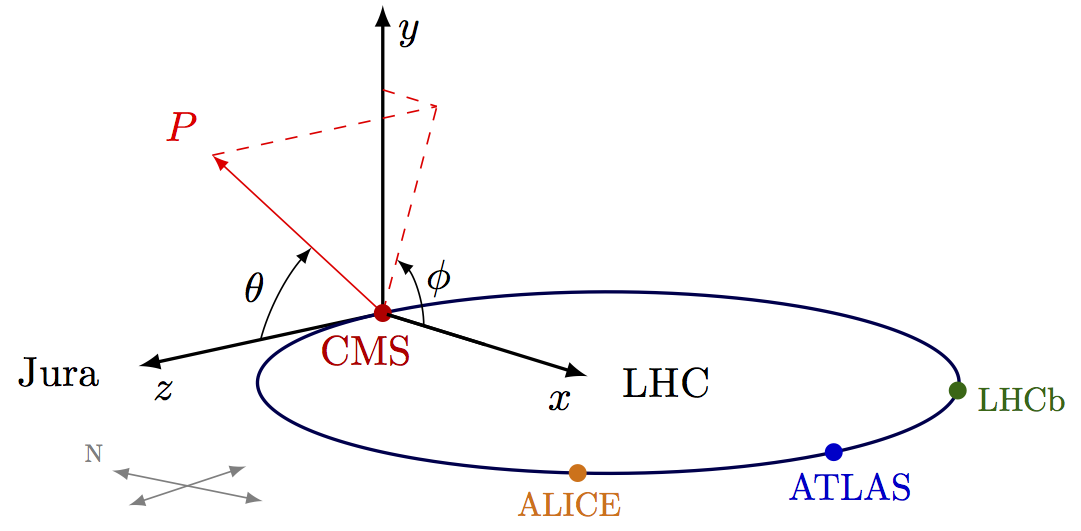
\includegraphics[width=0.8\textwidth]{Images/coordinatechart.png}
    \captionof{figure}{Coordinate system employed by the CMS experiment (retrieved from~\parencite{cmsplots}).}\label{fig_coordinates}
\end{center}

Throughout this work, phenomenological studies and comparisons are primarily developed in the context of CMS, although several results from ATLAS are also referenced, given the close alignment in sensitivity and scope. Measurements performed at CMS adopt a right-handed coordinate system with its origin at the nominal collision point. The $z$-axis is defined along the beam direction, the $x$-axis points radially inward toward the center of the LHC ring, and the $y$-axis points vertically upward. The azimuthal angle $\phi$ is measured in the transverse ($xy$) plane from the $x$-axis, while the polar angle $\theta$ is measured from the $z$-axis, as shown in Fig.~\ref{fig_coordinates}. Moreover, for kinematic analysis at hadron colliders, the Cartesian coordinate system is often reparameterized into quantities that are more physically meaningful and experimentally convenient as shown in Fig.~\ref{fig_cms_coor}:

\begin{description}
	\item[Pseudo-rapidity] $(\eta)$ Instead of using the polar angle, CMS measurements involve the pseudo-rapidity, defined by
	$$
	\eta=-\ln \left(\tan \frac{\theta}{2}\right)
	$$
	The main advantage of using the pseudo-rapidity is that distributions over it tend to be closer to a uniform distribution than those over the polar angle, see Fig.~\ref{fig_cms_coor}. Furthermore, the difference in pseudo-rapidity is invariant under Lorentz boosts along the beam direction~\parencite{book:1123430}.
	
	\item[Transverse Momentum] ($p_T$) Refers to the component of momentum which is perpendicular to the beam line. It is usually preferred over full momentum because momentum along the beamline may just be left over from the beam particles, while the transverse momentum is always associated with whatever physics happened at the vertex, see Fig.~\ref{fig_cms_coor}.
	
	\item[Azimuthal Angle] ($\phi$) Measures the angle in the transverse plane relative to the $x$-axis, providing the directional component perpendicular to the beam line.
\end{description}

\begin{center}
  		% CMS detector - left perspective
		\tdplotsetmaincoords{75}{50} % to reset previous setting
		\begin{tikzpicture}[scale=2.6,tdplot_main_coords,rotate around x=90]
			
			% VARIABLES
			\def\rvec{\L/2/cos(\thetavec)}
			\def\thetavec{18}
			\def\phivec{60}
			\def\L{3.3}    % detector length
			\def\R{0.75}   % detector cylinder radius
			\def\l{4.3}    % beam pipe length
			\def\r{0.04}   % beam pipe radius
			\def\rt{0.042} % beam pipe radius + line thickness
			\def\xmax{1}   % maximum x axis
			\def\ymax{1}   % maximum y axis
			\def\zmin{-\l/2-0.2} % minimum z axis
			\def\zmax{\l/2+0.3}  % maximum z axis
			\def\w{0.3}
			\coordinate (O) at (0,0,0);
			\coordinate (Z) at (0,0,\L/2);
			\tdplotsetcoord{O'}{0.022}{\thetavec}{\phivec} % slightly shifted origin
			\tdplotsetcoord{O''}{0.018}{90}{\phivec} % slightly shifted origin
			\tdplotsetcoord{P}{\rvec}{\thetavec}{\phivec}
			
			% CYLINDER behind
			\def\ang{19} % rotate lines to simulate cylinder
			\fill[top color=red!50!black!4,bottom color=red!60!black!2,rotate around z=\ang]
			(0,\R,\L/2) --++ (0,0,-\L) arc(90:270:\R) --++ (0,0,\L) arc(270:90:\R) -- cycle;
			\fill[detector surface] % transverse plane at z=L/2
			(0,0,\L/2) --++ (0,\R,0) arc(90:270:\R) -- cycle;
			\fill[detector surface] % transverse plane at z=-L/2
			(0,0,-\L/2) --++ (0,\R,0) arc(90:270:\R) -- cycle;
			\tdplotdrawarc[detector]{(0,0,\L/2)}{\R}{0}{360}{}{}
			\tdplotdrawarc[detector,thin]{(0,0,-\L/2)}{\R}{0}{360}{}{}
			%\draw[detector,canvas is yx plane at z=-\L/2] (0,0,0) circle(\R);
			\draw[detector,thin, dashed] % transverse plane at z=0
			(90-\ang:\R) arc (90-\ang:270:\R);
			\draw[detector] (0,0,-\L/2)++(90:\R) --++ (0,0,\L); % top horizontal
			\draw[detector] (0,0,-\L/2)++(-90:\R) --++ (0,0,\L); % bottom horizontal
			
			% BEAM PIPE
			\tdplotdrawarc[beam pipe]{(0,0,\l/2)}{\r}{0}{360}{}{}
			%\tdplotdrawarc[beam pipe]{(0,0,-\l/2)}{\r}{\ang-90}{90}{}{}
			%\draw[beam pipe] % cylindric beam pipe
			%  (0,\r,-\l/2) --++ (0,0,\l) arc(90:-90:\r)
			%  --++ (0,0,-\l) arc(-90:90:\r);
			\draw[beam pipe] % beam pipe, thinner in middle
			(0,\r,-\l/2) -- (0,\r,-0.2*\l) -- (90:0.5*\r)
			-- (0,\r,0.2*\l) -- (0,\r,0.5*\l) arc(90:-90:\r)
			-- (0,-\r,0.2*\l) -- (-90:0.5*\r) --
			(0,-\r,-0.2*\l) -- (0,-\r,-\l/2) arc(-90:90:\r);
			\draw[beam pipe] (0,0,\l/2) circle(\r);
			
			% AXES
			%\draw[thick,->] (0,0,0) -- (0,0,1) node[below right]{$z$}; % short
			\draw[axis,-] (0,0,\zmin) -- (0,0,0); % long
			\fill[CMScol] (O) circle(0.5pt) node[right=1,below=1] {IP};
			\draw[axis] (0,0,0.020) -- (0,0,\zmax) node[right=3,above=0.1]{$z$}; % long
			\draw[axis] (0,0.019,0) -- (0,\ymax,0) node[below left]{$y$};
			\draw[axis] (0.022,0,0) -- (\xmax,0,0) node[below=1,right=-2]{$x$};
			
			% LABELS
			\node[mydarkred,above] at (0,\ymax,0) {$\eta=0$};
			\node[mydarkred,above=0.6, left] at (0,\R,0.3*\L) {$\eta>0$};
			\node[mydarkred,above=0.7, right] at (0,\R,-0.2*\L) {$\eta<0$};
			\node[mydarkred,below=1,left] at (0,0,\zmax) {$\eta=\infty$};
			\node[mydarkred,above=1,right] at (0,0,\zmin) {$\eta=-\infty$};
			
			% VECTORS
			%\fill[radius=0.4,red] (P) circle;
			\draw[dashed,myred] (P)  -- (Pxy);
			\draw[dashed,myred] (Py) -- (Pxy);
			\draw[dashed,myred] (P) -- (Pz);
			
			
			\draw[->,miverde,line cap=round,draw opacity=0.9] (O') -- (P) node[anchor=-30] {\contour{white}{$\va*{p}$}};
			\draw[->,miverde,line cap=round] (O') -- (P) node[anchor=-30] {$\va*{p}$};
			
			\draw[->,azulF,line cap=round,draw opacity=0.9] (O') -- (Pxy) node[right, anchor=-100] {\contour{white}{$\va*{p}_T$}};
			% \draw[->,azulF,line cap=round] (O') -- (Pxy) node[right , anchor=-100] {$\va*{p}_T$};
			
			
			% CYLINDER front
			\draw[beam pipe,fill=none] (0,\r,-\l/2) arc(90:-90:\r);
			\fill[detector surface] % transverse plane at z=L/2
			(0,\rt,\L/2) --++ (0,\R-\rt,0) arc(90:-90:\R) --++ (0,\R-\rt,0) arc(-90:90:\rt);
			\fill[detector surface] % transverse plane at z=-L/2
			(0,\rt,-\L/2) --++ (0,\R-\rt,0) arc(90:-90:\R) --++ (0,\R-\rt,0) arc(-90:90:\rt);
			\tdplotdrawarc[detector]{(0,0,\L/2)}{\R}{-90}{90}{}{} % transverse plane at z=L/2
			\tdplotdrawarc[detector]{(0,0,-\L/2)}{\R}{-90}{90}{}{} % transverse plane at z=-L/2
			\draw[beam pipe,fill=none] (0,\r,\l/2) arc(90:-90:\r);
			\draw[detector,very thin, dashed] % transverse plane at z=0
			(90-\ang:\R) arc (90-\ang:-90:\R);
			
			% ANGLES
			\tdplotdrawarc[thick,red!57!black!3] % contour
			{(O)}{0.2}{4}{0.7*\phivec}{}{}

			% white to contour
			\tdplotdrawarc[draw=azulF, line width=0.6pt, draw opacity=0.9]{(O)}{0.2}{0}{\phivec}{above=2,right=0.75,anchor=-30,text=black}{\contour{white}{$\phi$}}
			\tdplotdrawarc[->, azulF]{(O)}{0.2}{0}{\phivec}{above=2,right=0.75,anchor=-30}{$\phi$}


			\tdplotdrawarc[->,rotate around z=\phivec-90,rotate around y=-90]
			{(O)}{0.88}{0}{\thetavec}{anchor=mid east}{$\theta$}
			\tdplotdrawarc[thick,red!58!black!4,rotate around z=\phivec-90,rotate around y=-90] % contour
			{(O)}{0.3}{88}{0.5*(90+\thetavec)}{}{}
			\tdplotdrawarc[-{>[flex'=1]},rotate around z=\phivec-90,rotate around y=-90,line cap=round]
			{(O)}{0.3}{90}{\thetavec}{above=4.5,right=0.5,anchor=mid east}{$\eta$}
			\draw[mydarkred] (0,0,\L/2) --++ (\R,0,0);
			\tdplotdrawarc[thick,red!60!black!6] % contour
			{(Z)}{0.2}{4}{0.7*\phivec}{}{}
			\tdplotdrawarc[draw=none,opacity=0.8]{(Z)}{0.2}{0}{\phivec}{above=2,right=0.7,anchor=-30}{\contour{red!60!black!6}{$\phi$}}
			\tdplotdrawarc[->]{(Z)}{0.2}{0}{\phivec}{above=2,right=0.7,anchor=-30}{$\phi$}
			
			% COMPASS - CMS-ATLAS axis has a ~12° declination (http://googlecompass.com)
			\begin{scope}[shift={(1.1*\R,-\R,0.2*\L)},rotate around y=12]
				\draw[<->,black!50] (-\w,0,0) -- (\w,0,0);
				\draw[<->,black!50] (0,0,-\w) -- (0,0,\w);
				\node[left,black!50,scale=0.6] at (-\w,0,0) {N};
				\node[below=3,left=-2,green!20!black!50,scale=0.6] at (0,0,\w) {Jura};
				%\node[below=1,right,black!50,scale=0.6,align=center] at (\w,0,0) {center of\\the LHC};
				%\node[below=1,right,blue!30!black!50,scale=0.6] at (\w,0,0) {ATLAS};
			\end{scope}
			\draw[->,thick,orange!30!black] (1.4*\w,-\R,-0.1*\L) --++ (2*\w,0,0)
			node[right,scale=0.8,align=center] {center of\\[-1pt]the LHC};
			
		\end{tikzpicture}
  \captionof{figure}{Detailed reparametrization of the coordinate system employed by the CMS experiment (retrieved from~\parencite{cmsplots})}\label{fig_cms_coor}
\end{center}

Together, the triplet $(p_T, \phi, \eta)$ forms a natural coordinate system that fully describes a particle's three-momentum vector at a hadron collider. The full four-momentum $(E, p_x, p_y, p_z)$ can be reconstructed from these quantities, typically supplemented by either the particle's mass hypothesis (for identified particles like electrons or muons) or the energy deposited in the calorimeters (for neutral objects like photons or jets). This $(p_T, \phi, \eta)$ system serves as the fundamental framework for defining physical objects, calculating event variables, and performing analyses at the LHC, providing both experimental convenience and physical insight into the collision dynamics.


A key challenge is isolating the primary hard interaction from the additional concurrent pile-up interactions. This is accomplished by reconstructing distinct interaction vertices along the beam direction and associating charged particles to their point of origin. The ultimate aim of the reconstruction chain is to identify all stable particles produced in the collision and measure their four-momenta, thereby enabling the identification of the underlying fundamental process.

However, the reconstruction is complicated by several factors. The initial state of the colliding protons is not fully known, as they are composite particles made up of quarks and gluons (collectively referred to as partons). The fraction of the proton's momentum carried by each parton is described by parton distribution functions (PDFs), which are determined experimentally. Consequently, the total momentum along the beam axis ($z$) is not balanced on an event-by-event basis. Furthermore, not all particles are stable enough to reach the detector; some decay before being detected, and only their decay products are observed. The design of a collider experiment, illustrated in Fig.~\ref{fig_layers}, is optimized for the identification and energy measurement of the particles produced in high-energy collisions.

\begin{center}
    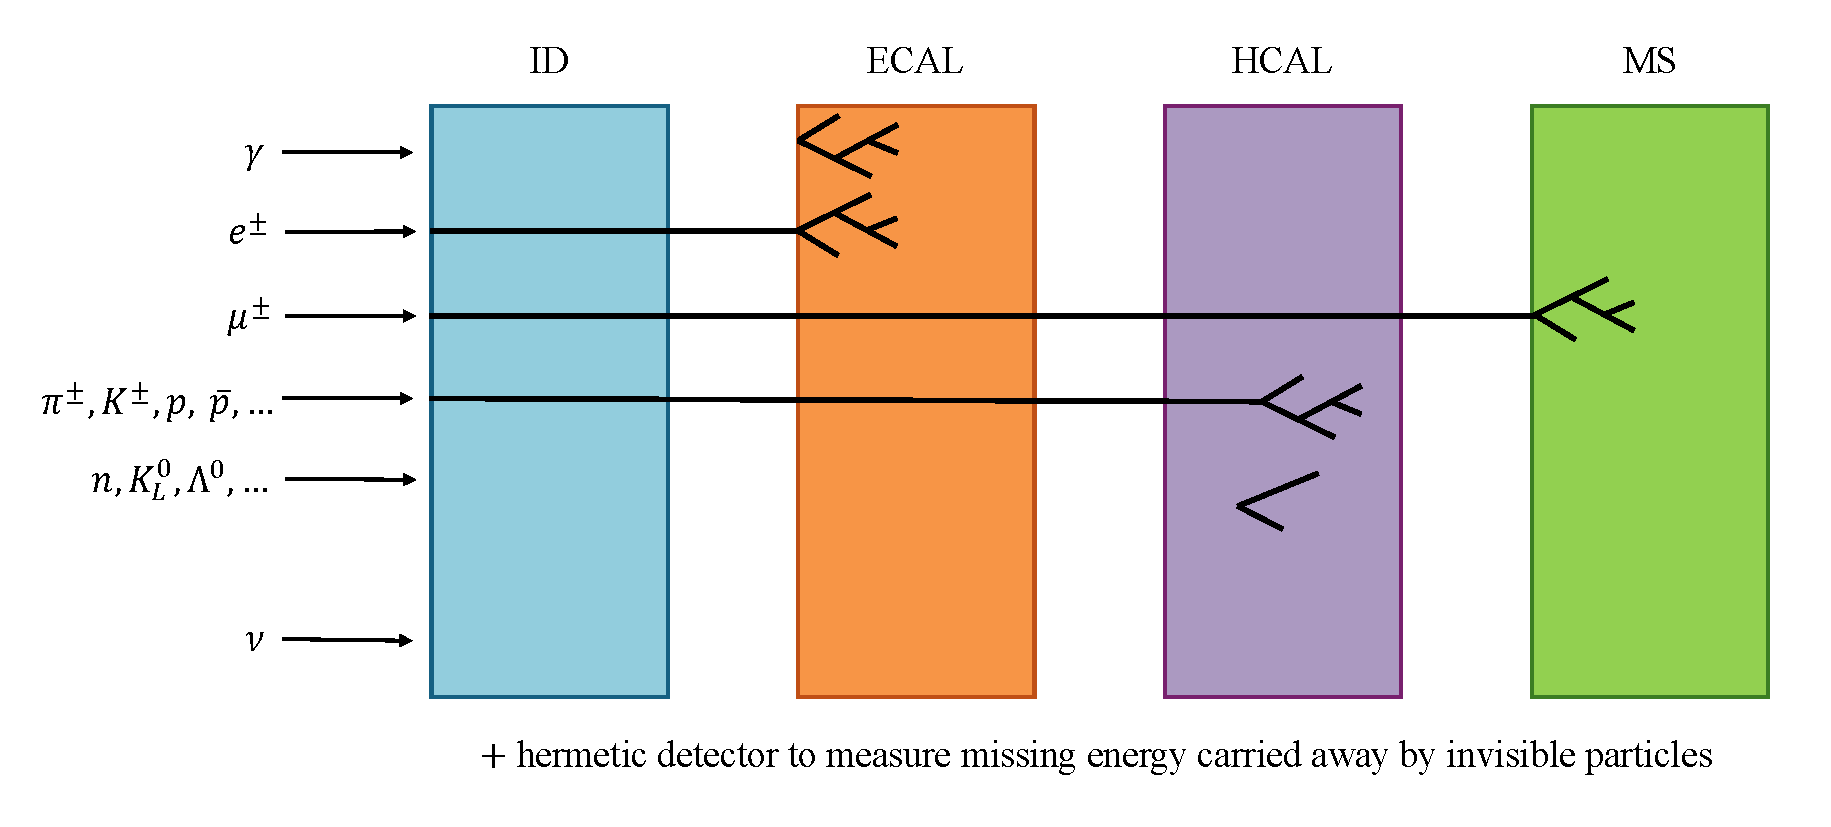
\includegraphics[width=0.95\textwidth]{Images/Layers.pdf}
    \captionof{figure}{Illustration of high-energy particles being identified by consecutive types of subdetectors in a typical collider experiment. The curvature of the tracks in the magnetic field is not shown for simplicity. Representation of which particles and kinds of detectors are used in a multipurpose detector such as CMS or ATLAS.}\label{fig_layers}
\end{center}

Finally, some hypothetical particles, such as those comprising dark matter, along with known neutrinos, interact very weakly with matter and escape direct detection. Therefore, a hermetic detector design is crucial to infer their presence by accurately measuring the imbalance of energy and momentum in the transverse plane, referred to as missing transverse momentum.


In this way, a typical collider experiment comprises several main detector subsystems that are used jointly to detect and measure the properties of particles produced in the collision. A \textit{schematic representation} of such a generic multipurpose detector is shown in Fig.~\ref{fig_detector}. The detector features an "onion-like" design of several concentric layers, each optimized to identify different types of particles and measure their properties.

\begin{center}
    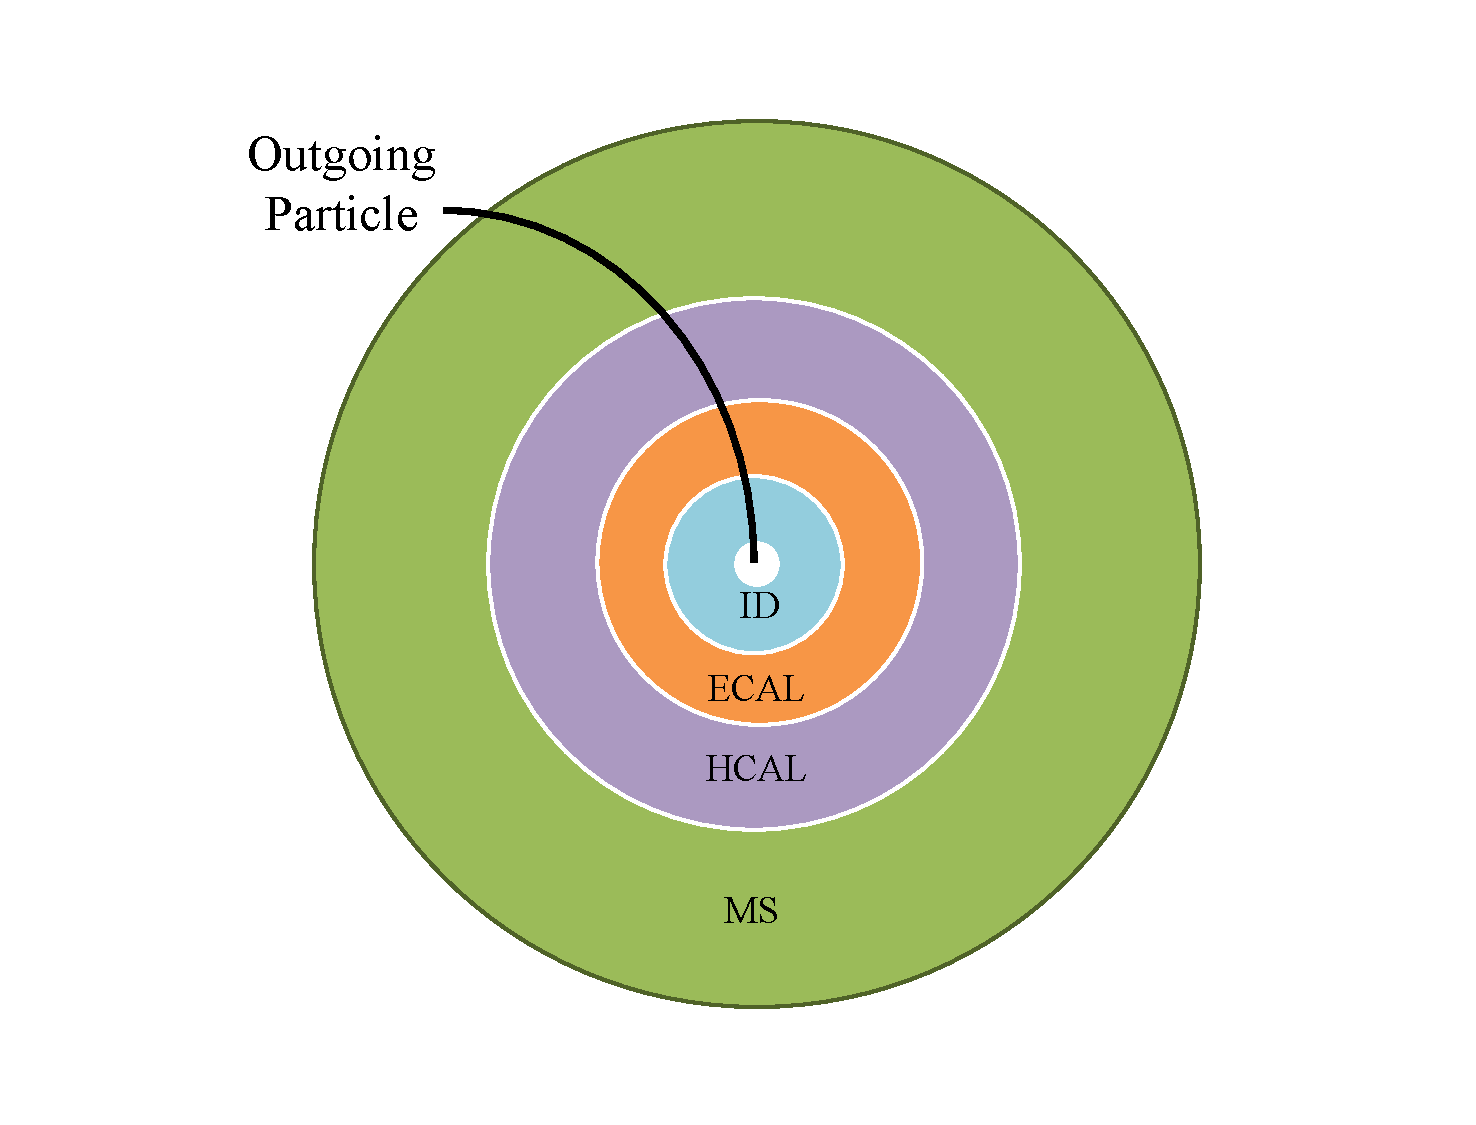
\includegraphics[width=0.8\textwidth]{Images/transversal_detector.pdf}
    \captionof{figure}{Schematic representation of a transverse section of a generic multipurpose detector. The inner detector (ID) is used to measure the trajectories of charged particles, the electromagnetic calorimeter (ECAL) measures the energy of photons and electrons, the hadronic calorimeter (HCAL) measures the energy of hadrons, and the muon system (MS) identifies and measures muons. The missing transverse momentum (MET) is inferred from the momentum imbalance in the transverse plane.}\label{fig_detector}
\end{center}

The innermost subsystem, the inner detector (ID) or tracker, is immersed in a strong axial magnetic field (typically 1–4 T). It is designed to reconstruct the trajectories of charged particles, which are bent by the magnetic field. The direction and curvature of these trajectories, called \textbf{tracks}, yield the particle's momentum vector and electric charge. The most common long-lived charged particles from the SM are leptons (electrons $e$ and muons $\mu$) and hadrons (pions $\pi$, kaons $K$, and protons $p$). In some detectors, the ID is complemented by a Cherenkov-light detector to measure particle velocity. Combined with the momentum measurement, this velocity helps determine the particle mass, allowing for differentiation between pions, kaons, and protons.

After the tracker, particles enter the electromagnetic calorimeter (ECAL), which is designed to fully absorb photons, electrons, and positrons. These particles deposit all their energy in the ECAL by initiating an electromagnetic shower via bremsstrahlung and $e^{+}e^{-}$ pair production. Electrons are identified as charged tracks that point to a compact, high-energy deposit in the ECAL.

The hadronic calorimeter (HCAL) surrounds the ECAL. Its purpose is to absorb hadrons (e.g., neutrons, protons, pions, kaons) and measure their energy through hadronic interactions. High-energy quarks and gluons do not appear as individual particles but instead \textbf{hadronize} into collimated sprays of hadrons known as \textbf{jets}, see Sec.~\ref{sec:jets}. A jet's energy is measured by combining the energy deposited in the ECAL and HCAL with the momenta of charged tracks associated with it. This approach, known as particle flow (PF) reconstruction, provides a more accurate measurement. Neutral hadrons are identified as energy deposits in the calorimeters with no associated track in the ID.

Muons are unique as they are the only charged particles (apart from neutrinos) that can penetrate the entire calorimeter system, losing only a small amount of energy via ionization. Therefore, a dedicated muon system (MS) is built outside the calorimeters. Muons are identified as tracks in the ID that are matched to tracks in the MS. The MS, often within its own magnetic field, provides a standalone momentum measurement, which is combined with the ID measurement for high precision.

Since the detector is nearly hermetic (covering almost the full solid angle), momentum conservation in the plane transverse to the beam line ($x$-$y$ plane) is a powerful tool. The vector sum of the momenta in the transverse plane ($\vec{p}_T$) of all detected particles should be zero. Any significant imbalance indicates the presence of undetected, neutral particles that did not interact with the detector, such as neutrinos or hypothetical new particles. This imbalance is called missing transverse momentum (MET) and is formally defined as:
$$
\vec{p}_T^{\text{miss}} \equiv -\sum_i \vec{p}_{T,i}
$$
where the sum runs over all reconstructed particles (e.g., leptons, photons, jets) or calorimeter deposits in the event.

This sophisticated detector design, optimized for identifying and measuring Standard Model particles, also makes it a powerful instrument for searching for new physics beyond the SM through unusual signatures or an excess of events with large MET.


The event rate $R$ for a physical process (e.g., $pp \to X$) is governed by the accelerator's luminosity $\mathcal{L}$ and the process cross section $\sigma$. Luminosity quantifies the performance of a collider to produce interactions, establishing the proportionality,
\begin{equation}
	\frac{d R}{d t} = \mathcal{L} \sigma,
\end{equation}
where $\sigma$ (typically measured in barns, $1\,\text{b} = 10^{-24}\,\text{cm}^2$) encodes the interaction probability. For LHC proton bunches colliding head-on with Gaussian transverse profiles, the instantaneous luminosity is~\parencite{Herr:941318,book:1123430}:
\begin{equation}
	\mathcal{L} = \frac{f N_{b}}{4\pi} \frac{N_{1} N_{2}}{\sigma_{x} \sigma_{y}}\label{eq_lumi}
\end{equation}
Here, $N_{1,2}$ are proton counts per bunch, $f$ is the bunch collision frequency, $N_{b}$ is the number of bunches, and $\sigma_{x,y}$ are transverse beam widths. 

Integrating $\mathcal{L}$ over time yields the total integrated luminosity $L$, linking directly to the observed event count $N$:
\begin{equation}
	L = \int \mathcal{L}\, dt \quad \Rightarrow \quad N = L \sigma.
\end{equation}

%This major upgrade aims to increase the integrated luminosity by more than an order of magnitude, targeting up to $3\,\mathrm{ab}^{-1}$ of data per experiment. The HL-LHC will significantly enhance the sensitivity to rare processes, improve the precision of Standard Model measurements, and boost the discovery potential for BSM phenomena.

  
The Gaussian beam approximation in~\eqref{eq_lumi} ignores hourglass effects (beam divergence near interaction points) and dynamic $\sigma_{x,y}$ variations during fills. CMS mitigates these via real-time luminosity monitoring using pixel clusters~\parencite{Sirunyan2021}, with systematic uncertainties below $2\%$. High $\mathcal{L}$ also introduces pileup—multiple $pp$ interactions per bunch crossing—which complicates $\eta$/$\phi$ measurements but is corrected using vertex isolation algorithms.


The following variables are related to the particles being produced rather than the accelerator.
\begin{description}
	\item[Decay width] ( $\Gamma)$ The decay rate is the probability that a given particle will decay per unit time. Since a particle can have multiple decay modes, the total decay rate is the sum of the decay rates for each mode~\parencite{book:1123430}. The relative frequency of a decay mode is the branching ratio, given by
	$$
	\mathrm{BR}(j)=\frac{\Gamma(j)}{\Gamma} .
	$$
	\item[Cross-section] $(\sigma)$ The cross-section is a measure of the probability that an interaction will occur from a collision. It is a quantum-mechanical analogue of the "effective size" of the particles involved in an interaction.

	\item[Pseudo-rapidity] $(\eta)$ Instead of using the polar angle, CMS measurements involve the pseudo-rapidity, defined by
	$$
	\eta=-\ln \left(\tan \frac{\theta}{2}\right)
	$$
	The main advantage of using the pseudo-rapidity is that distributions over it tend to be closer to a uniform distribution than those over the polar angle, see Fig.~\ref{fig_cms_coor}. Furthermore, the difference in pseudo-rapidity is invariant under Lorentz boosts along the beam direction~\parencite{book:1123430}.
	\item[Transverse Momentum] ($p_T$) Refers to the component of momentum which is perpendicular to the beam line. It is usually preferred over full momentum because momentum along the beamline may just be left over from the beam particles, while the transverse momentum is always associated with whatever physics happened at the vertex, see Fig.~\ref{fig_cms_coor}.
	\item[Missing transverse energy and momentum] $\left(E_{T}^{\text {miss }} \& p_{T}^{\text {miss }}\right)$ Missing energy and momentum refers to the energy and momentum that is not detected but is expected to be there as a consequence of energy conservation and momentum conservation. This momentum is often carried by particles that do not interact electromagnetically or strongly and are therefore difficult to detect~\parencite{book:1123430}. Missing energy and momentum provides an indirect measurement of undetectable particles in hadron colliders such as neutrinos. Missing momentum reconstructions focus on the transverse direction, where total momentum is expected to be zero.
\end{description}

 
\section{Jets Reconstruction}\label{sec:jets}

Quarks and gluons are never observed as free particles because of colour confinement~\cite{Andersson:1983,Webber:1984}. Nevertheless, perturbative QCD treats them as the relevant short-distance degrees of freedom: factorization theorems and asymptotic freedom justify computing hard-scattering matrix elements for incoming and outgoing partons even though QCD becomes non-perturbative at low scales~\cite{Collins:1989}. The strong coupling $\alpha_s$ grows large and effectively ``blows up'' around the confinement scale $\Lambda_{\mathrm{QCD}}$~\cite{1674-1137-40-10-100001}; consequently, something must happen to quarks and gluons before they reach the detector~\cite{Sjostrand:2014zea}. In practice, the gluon and all quarks except the top hadronize, producing cascades of baryons and mesons that themselves undergo further decays; hadronization is modelled e.g. with the Lund string or cluster models~\cite{Andersson:1983,Webber:1984,Sjostrand:2014zea}. At the LHC, these hadrons typically carry energies comparable to the electroweak scale, and relativistic boosts tend to collimate their decay products into narrow bunches~\cite{Salam:2010}. Those collimated collections of hadrons are the jets we measure at hadron colliders and the objects we use to infer the partons produced in the hard interaction~\cite{Salam:2010,Cacciari:2008gp}.

Each high-energy parton produced in a collision, such as a quark from the process $gg \rightarrow q\bar{q}$, undergoes hadronization over a distance scale of~$\sim10^{-15}\,\mathrm{m}$, producing a jet of hadrons~\cite{Andersson:1983,Sjostrand:2014zea}. The energy composition of these jets is phenomenologically well established and is the basis of particle‑flow reconstruction: on average roughly $\sim60\%$ of the jet energy is carried by charged particles (mostly $\pi^{\pm}, K^{\pm}$), $\sim30\%$ by photons (from $\pi^0\to\gamma\gamma$) and $\sim10\%$ by neutral hadrons~\cite{CMS:PF2017}. In high-energy jets, the particles can be too collimated to be resolved individually in coarse calorimeter segmentation; nevertheless, the jet four‑momentum is reconstructed from clustered PF candidates or calorimeter deposits and then corrected using jet energy corrections derived from simulation and in‑situ data~\cite{CMS:PF2017,Cacciari:2011ma,deFavereau:2013fsa}.

Phenomenologically one usually assumes that each high-energy parton yields a jet and that the measured jet four-momentum can, to useful accuracy, be related to the original parton four-momentum~\cite{Catani:1993,Ellis:1993}. Jets are therefore defined operationally using recombination (clustering) algorithms such as Cambridge–Aachen~\cite{Dokshitzer:1997} or the (anti‑)kT family~\cite{Cacciari:2008gp}. Experimentally this means grouping a large number of energy depositions (or particle‑flow candidates) observed in the calorimeters and tracker into a much smaller set of jets or sub‑jets~\cite{CMS:PF2017}. Nothing in the raw detector data, however, indicates a priori how many jets there should be: the clustering procedure and the choice of a resolution scale fix the outcome~\cite{Salam:2010}. In practice one must either specify the desired number of final jets or choose a resolution/stop criterion (for example a distance parameter $R$, a clustering distance cut, or a jet‑mass/sub‑jet‑resolution threshold) that determines the smallest substructure to be considered a separate parton‑like object~\cite{Thaler:2011}.

Modern reconstruction at the LHC typically uses particle‑flow (PF) candidates as input together with infrared‑ and collinear‑safe clustering algorithms to define jet four‑momenta~\cite{CMS:PF2017,Cacciari:2011ma}. The anti‑$k_T$ algorithm~\cite{Cacciari:2008gp}, implemented in \texttt{FastJet}~\cite{Cacciari:2011ma}, is widely used in ATLAS and CMS; it groups candidates by proximity in the rapidity–azimuth $(y,\phi)$ plane with a typical distance parameter $R\sim0.4$–0.6 and is relatively insensitive to soft radiation and pileup when combined with area‑based subtraction techniques~\cite{Cacciari:2008area}. After clustering, jet energy corrections (JEC) derived from simulation and in‑situ calibrations compensate for detector response, pileup, and underlying‑event effects~\cite{CMS:JEC}, while jet‑substructure and tagging algorithms (mass‑drop, N‑subjettiness, SoftDrop, etc.) help infer the flavour and origin of the initiating parton~\cite{Butterworth:2008,Thaler:2011,Larkoski:2014}.


\subsection{Jet algorithms}

Recombination (or sequential clustering) algorithms formalise the intuitive idea that parton showering produces collinear and soft splittings~\cite{Catani:1993,Dokshitzer:1997,Salam:2010}: two nearby and kinematically compatible sub-jets are merged if they are more likely to have originated from a single parton~\cite{Catani:1993,Dokshitzer:1997}. A practical implementation requires a measure of ``distance'' between objects~\cite{Catani:1993,Cacciari:2011ma}; common choices combine an angular separation in the rapidity–azimuth plane, $\Delta R_{ij}$, with a transverse-momentum weighting~\cite{Catani:1993,Cacciari:2008gp}. Typical distance measures are~\cite{Catani:1993,Dokshitzer:1997,Cacciari:2008gp}
\begin{equation}
  \begin{array}{lll}
  k_T: & y_{ij}=\dfrac{\Delta R_{ij}}{R}\min(p_{T,i},p_{T,j}), & y_{iB}=p_{T,i},\\[6pt]
  \mathrm{C/A}: & y_{ij}=\dfrac{\Delta R_{ij}}{R}, & y_{iB}=1,\\[6pt]
  \text{anti-}k_T: & y_{ij}=\dfrac{\Delta R_{ij}}{R}\min(p_{T,i}^{-1},p_{T,j}^{-1}), & y_{iB}=p_{T,i}^{-1}.
  \end{array}  
\end{equation}
The parameter $R$ balances jet–jet and jet–beam criteria and sets the geometric size of jets; in LHC analyses, typical values are $R\sim0.4\text{--}0.7$ depending on the physics target~\cite{Cacciari:2011ma}.

Two operational modes are useful to distinguish. In an exclusive algorithm, one supplies a resolution scale $y_{\text{cut}}$ and proceeds iteratively:
\begin{enumerate}
  \item compute $y^{\min}=\min_{i,j}\{y_{ij},y_{iB}\}$;
  \item if $y^{\min}=y_{ij}<y_{\text{cut}}$ merge $i$ and $j$ and repeat;
  \item if $y^{\min}=y_{iB}<y_{\text{cut}}$ remove $i$ as beam radiation and repeat;
  \item stop when $y^{\min}>y_{\text{cut}}$ and keep remaining sub-jets as jets.
\end{enumerate}
An inclusive algorithm omits $y_{\text{cut}}$ and instead declares a sub-jet a final-state jet when its jet–beam distance is the smallest quantity; iteration continues until no inputs remain. Inclusive algorithms therefore produce a variable number of jets, while exclusive algorithms deliver a scale-dependent fixed set.

A practical question is how to combine the kinematics of merged objects. The most common choice in modern experiments is the E-scheme: four-vectors are added, which preserves energy–momentum and yields a physical jet mass useful for substructure and boosted-object tagging. An alternative is to sum three-momenta and rescale the energy to enforce a massless jet; this can be appropriate when the analysis targets massless parton kinematics, but it discards potentially useful jet-mass information.

From a theoretical and experimental viewpoint, important properties are infrared and collinear safety: a jet algorithm should give stable results under the emission of soft particles or collinear splittings. The $k_T$, C/A and anti-$k_T$ families are constructed to satisfy these requirements. Their practical behavior differs: $k_T$ naturally follows the physical shower history soft-first clustering, C/A is purely geometric useful for declustering and substructure studies, while anti-$k_T$ produces regular, cone-like jets that are robust and convenient experimentally.

Corrections for pileup and the underlying event are necessary at the LHC. These corrections depend on the jet area and are typically performed by estimating an event-wide transverse-momentum density and subtracting the corresponding contribution proportional to the jet area. Finally, because inclusive algorithms can produce jets arbitrarily close to the beam, a minimum jet $p_T$ threshold, commonly 20–100 GeV depending on the analysis, is imposed to ensure experimental observability and theoretical control.

\subsection{$\tau$ Tagging at Multipurpose Detectors}

The $\tau$ lepton decays hadronically with a probability of $\sim65\%$, producing a narrow ``$\tau$-jet'' that contains only a few charged and neutral hadrons~\cite{1674-1137-40-10-100001,CMS:2018jrd}. Hadronic decays are dominated by one- and three-prong topologies and often include neutral pions that promptly convert to photons, giving a sizable electromagnetic fraction in the calorimeters~\cite{1674-1137-40-10-100001,ATLAS:2014rzk}. When the $\tau$ momentum is large compared to its mass the decay products are highly collimated~\cite{CMS:2018jrd,CMS_DeepTau}: for $p_T>50\ \mathrm{GeV}$ roughly $90\%$ of the visible energy is contained within a cone of radius $R=\sqrt{(\Delta\eta)^2+(\Delta\varphi)^2}=0.2$~\cite{CMS:2018jrd}. These properties motivate the use of small signal cones and narrow isolation annuli in reconstruction~\cite{CMS:2018jrd,CMS_DeepTau}.

Identification exploits three complementary classes of observables~\cite{CMS:2018jrd,ATLAS:2014rzk,CMS_DeepTau,CMS:PF2017}:

\begin{itemize}
  \item Calorimetric isolation and shower-shape variables~\cite{CMS:2018jrd,ATLAS:2014rzk}: hadronic $\tau$ decays deposit localized energy in ECAL+HCAL~\cite{CMS:2018jrd}. Experiments use isolation sums and shape ratios to quantify peripheral activity~\cite{CMS:2018jrd,ATLAS:2014rzk}. Example variables are
  \begin{equation}
    \Delta E_T^{12}=\frac{\sum_{\;0.1<\Delta R<0.2} E_{T,j}}{\sum_{\;\Delta R<0.4} E_{T,i}},\;\;
    P_{\mathrm{ISOL}}=\sum_{\Delta R<0.40}E_T - \sum_{\Delta R<0.13}E_T,
  \end{equation}
  which suppress QCD jets that populate the isolation ring~\cite{CMS:2018jrd}.
  \item Charged-track isolation and prong topology~\cite{CMS:2018jrd,CMS:PF2017}: the few, collimated charged tracks of a $\tau$ allow powerful selections. A common procedure defines a matching cone of radius $R_{\mathrm{m}}$ around the calorimeter jet axis to select candidate tracks above a $p_T^{\min}$ threshold; the leading track (tr$_1$) defines a narrow signal cone $R_{\mathrm{S}}$ (1- or 3-prong hypotheses) and a larger isolation cone $R_{\mathrm{I}}$ is scanned for additional tracks~\cite{CMS:2018jrd,CMS:PF2017}.
  \item Lifetime and vertexing observables~\cite{CMS:TRK2014,1674-1137-40-10-100001}: the finite $\tau$ lifetime ($c\tau\approx87\ \mu\mathrm{m}$) produces displaced tracks and, for multi-prong decays, a reconstructible secondary vertex; impact-parameter significances and secondary-vertex properties are exploited to separate genuine $\tau_h$ from prompt jets or leptons~\cite{CMS:TRK2014,1674-1137-40-10-100001}.
\end{itemize}


Additional discriminants include the invariant mass of the visible decay products computed from tracks and calorimeter clusters, electromagnetic energy fractions (sensitive to $\pi^0\to\gamma\gamma$), and dedicated shower-strip grouping for nearby photons. For example, invariant-mass reconstruction commonly uses a jet cone $\Delta R_{\text{jet}}\lesssim0.4$ while excluding calorimeter clusters matched to tracks by a minimum separation $\Delta R_{\text{track}}\gtrsim0.08$ to reduce double counting.

Reconstruction algorithms combine these inputs. CMS's Hadron-Plus-Strips (HPS) and modern DeepTau methods explicitly build decay-mode hypotheses and use strip-clustering of photons plus multivariate or deep-learning discriminators to reject jets, electrons, and muons~\parencite{CMS:2022ydz,CMS_DeepTau}. ATLAS employs analogous calorimeter+track based MVAs and BDTs~\parencite{ATLAS:2022fgo}. Typical working points trade efficiency versus background: medium points often give $\tau_{\mathrm{h}}$ efficiencies of order 50–70\% with light-jet misidentification rates in the per-mille to percent range, depending on kinematics and pileup.

Practical implementations tune cone sizes, isolation thresholds, and MVA inputs to the kinematic region and analysis goals; the choice of working point is driven by the signal-to-background optimization for the search or measurement at hand.


\subsection{B Tagging at Multipurpose Detectors}

Jets originating from bottom quarks ($b$-jets) exhibit several distinctive properties that enable their identification. The relatively long lifetime of $b$ hadrons (order 1.5 ps) produces displaced charged tracks and often reconstructible secondary vertices a few millimetres from the primary interaction point. The large $b$-hadron mass yields decay products with sizable transverse momentum relative to the jet axis, and semileptonic branching fractions produce soft electrons or muons inside the jet. These features form the basis for $b$-tagging~\cite{CMS_BTV2016}.

Practical algorithms exploit individual signatures or combine them:
\begin{itemize}
  \item \textbf{Track-counting:} counts tracks with large impact-parameter significance to identify a $b$-like topology~\cite{CMS_BTV2016}.
  \item \textbf{Jet-probability:} evaluates the compatibility of the jet's track impact-parameter distribution with the primary vertex hypothesis~\cite{CMS_BTV2016}.
  \item \textbf{Secondary-vertex:} explicitly reconstructs displaced vertices and uses their kinematic properties (decay length significance, vertex mass)~\cite{CMS_BTV2016}.
  \item \textbf{Soft-lepton taggers:} identify low-$p_T$ leptons inside jets from semileptonic $b$ decays~\cite{CMS_BTV2016}.
\end{itemize}

Modern taggers combine many observables in multivariate or deep learning classifiers to maximize discrimination power. Contemporary approaches exploit rich, low level inputs (track by track and PF candidate information, vertex features and kinematics) and advanced network architectures (DeepCSV/DeepJet, RNN/sequence, graph/set networks)~\cite{CMS_BTV2016,Bols_2020,ATLAS:2022fgo}. These developments yield measurable performance gains: modern deep classifiers typically improve $b$ efficiency at fixed mistag rate relative to classical taggers, and allow continuous discriminants with tunable operating points. Calibration with data-driven scale factors (from $t\bar t$, multijet or dilepton control samples) and propagation of associated systematic uncertainties remain essential for physics results~\cite{CMS_BTV2016}.


\begin{itemize}
  \item Deep feed-forward networks (e.g. DeepCSV/DeepJet) ingest a large set of high-level and per-track inputs to produce powerful binary or multi-class discriminants that separate $b$, $c$ and light-flavour jets.
  \item Sequence models and recurrent networks (RNN-based taggers) process an arbitrary ordered list of track-level variables, improving sensitivity by directly exploiting per-track correlations and order-dependent information (impact-parameter sequences, track kinematics).
  \item Graph- and set-based architectures and combined particle+vertex networks (sometimes referred to as ``DeepFlavour''-style models) aggregate heterogeneous inputs and return per-flavour probabilities, enabling natural multi-classification and calibrated operating points.
\end{itemize}

These developments yield measurable performance gains: modern deep classifiers typically improve $b$ efficiency at fixed mistag rate (or reduce mistag rates at fixed efficiency) relative to classical taggers. The continuous output of such networks permits analyses to choose operating points (loose/medium/tight) corresponding to desired efficiencies or mistag targets. Calibration remains essential: data-driven scale factors derived from control samples (e.g. $t\bar t$, multijet, dilepton) are applied to correct simulation, and systematic uncertainties from the calibration, flavour composition, and kinematic extrapolation are propagated to physics results.

Examples in use are CMS DeepCSV / DeepJet and ATLAS MV2 / DL1~\parencite{CMS_DeepTau,ATLAS:2022fgo}, which illustrate the transition from expert-designed high-level variables to large-scale machine learning leveraging low-level detector information. Typical medium working points yield $b$-tag efficiencies of order 60–80\% with light-jet misidentification rates at or below the percent level; the precise choice of working point is tuned per analysis to optimise sensitivity while accounting for calibration and systematic uncertainties.

\section{The CMS Detector}

CMS is a general-purpose detector at the LHC~\parencite{CMS_2008}. With a length of 21.6~m, a diameter of 14.6~m, and a weight of 14,000 tonnes, its cylindrical geometry is divided into a central barrel section and two endcaps. This design provides hermetic coverage to accurately measure momentum and energy balance, which is crucial for identifying non-interacting particles like neutrinos through missing transverse energy.



The detector is constructed from concentric layers of sub-detectors, as illustrated in Figure~\ref{fig_cms}. The innermost component is the silicon tracker, comprising a pixel detector and silicon strip tracker. It reconstructs the trajectories of charged particles and measures their transverse momenta ($p_T$) with a resolution of $\approx 0.7\%$ for 10~GeV particles within a pseudorapidity range of $|\eta| < 2.5$.

Surrounding the tracker is the calorimetric system. The electromagnetic calorimeter (ECAL) is made of lead-tungstate crystals. It is designed to measure electrons and photons with a high resolution of $\approx 0.6\%$ for 50~GeV electrons. The hadronic calorimeter (HCAL), located outside the ECAL, is a brass-scintillator sampling calorimeter that measures hadrons (e.g., charged pions, kaons, protons) with an energy resolution of $\approx 18\%$ for 50~GeV pions. Together, the ECAL and HCAL cover $|\eta| < 3$. The coverage is extended to $|\eta| < 5$ with steel and quartz-fiber hadron calorimeters in the forward regions.


\begin{center}
	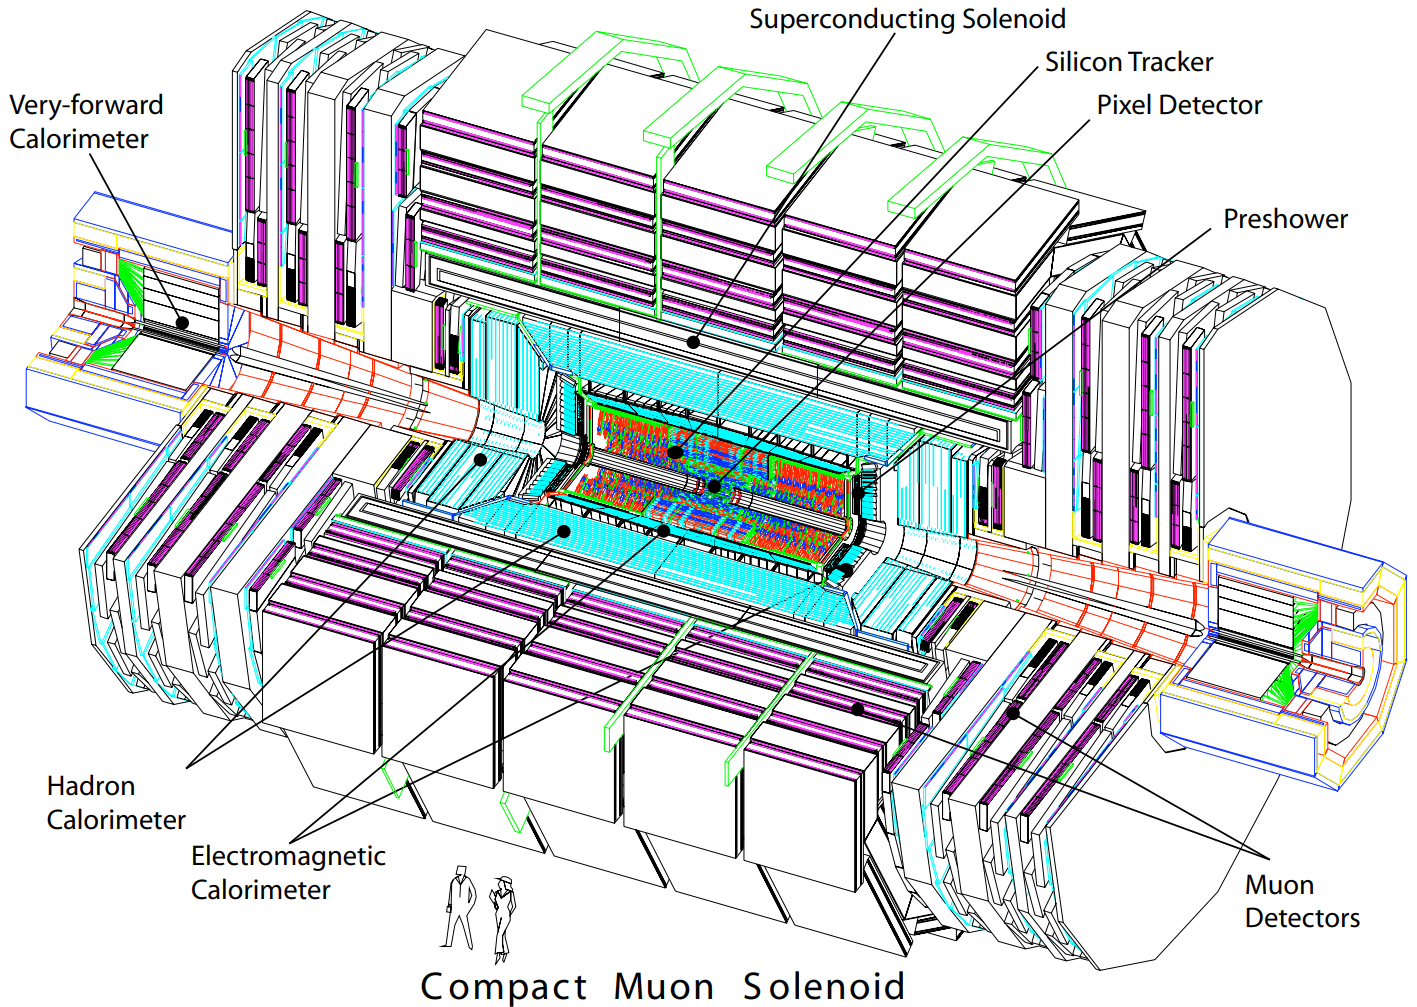
\includegraphics[width=0.9\textwidth]{Images/CMS.png}
	\captionof{figure}{Layout of the CMS experiment at the CERN LHC. (retrieved from~\parencite{CMS_2008}).}\label{fig_cms}
\end{center}

A key feature of CMS is its large superconducting solenoid, which encloses the tracker and calorimeters. The solenoid is constructed from a niobium-titanium alloy and cooled to 4.2~K with liquid helium. It generates a uniform magnetic field of 3.8~T throughout the tracking volume, enabling precise momentum measurement from the curvature of charged particle tracks.

The outermost system is dedicated to muon identification and measurement. Gas-ionization detectors are embedded in the steel flux-return yoke that surrounds the solenoid. This system provides triggering and tracking capabilities for muons up to $|\eta| < 2.4$. The combination of the inner tracker and the muon system allows for a robust identification and momentum measurement of muons across a wide kinematic range.

The geometrical segmentation of the barrel and endcaps defines the detector's acceptance in terms of pseudorapidity. The central barrel provides optimal coverage for $|\eta| \lesssim 1.5$, while the endcaps extend the acceptance to $|\eta| \lesssim 2.5$ for the tracker and calorimeters, and to $|\eta| \lesssim 2.4$ for the muon system.

This segmentation impacts the detection efficiency. The silicon trackers are highly efficient in the barrel, where particles cross the layers perpendicularly. In the endcaps, the reduced hit multiplicity from shallow-angle traversals leads to a slight decrease in tracking efficiency and resolution. The calorimeters are also optimized to maintain performance across $\eta$, though the material budget and granularity vary.

Muon reconstruction performance exhibits regional differences. In the barrel, drift tubes (DTs) provide high spatial resolution, while in the endcaps, cathode strip chambers (CSCs) and resistive plate chambers (RPCs) are used to handle higher background rates and non-uniform magnetic fields. The assumed identification efficiency for muons (electrons) is 95\% (85\%), with a mis-identification rate of 0.3\% (0.6\%)~\parencite{CMS-PAS-FTR-13-014,CMS_MUON_17001,CMS_EGM_17001}.

For the identification of heavy-flavor jets, we adopt the DeepCSV algorithm~\parencite{CMS_BTV2016}. We use its ``medium'' working point, which provides a $b$-tagging efficiency of 70\% with a light-flavor jet misidentification rate of approximately 1\% across the entire $p_T$ spectrum. The ``loose'' (85\% efficiency, 10\% mis-id) and ``tight'' (45\% efficiency, 0.1\% mis-id) working points were also explored during the analysis optimization.

For hadronically decaying $\tau$ leptons ($\tau_h$), we use the DeepTau algorithm~\parencite{CMS_DeepTau}, which employs a deep neural network combining isolation and lifetime information to identify $\tau_h$ decay modes. The ``medium'' working point is chosen for this analysis, providing a $\tau_h$ identification efficiency of 70\% and a misidentification rate of 0.5\% for jets originating from light quarks and gluons. This working point was selected through an optimization process that maximized the discovery reach of the analysis.
 
\section{The Phenomenological Pipeline: From Theory to Observables}

The estimation of signal and background event yields is performed through a comprehensive Monte Carlo (MC) simulation pipeline. This approach, a cornerstone of high-energy physics research, enables robust studies of Beyond the Standard Model (BSM) scenarios by emulating the entire data collection and processing chain of a collider experiment. The key advantages of this methodology include:

\begin{itemize}
    \item The ability to perform automated calculations of theoretical quantities such as cross-sections and decay widths for complex processes.
    \item Conducting feasibility studies and optimizing analysis strategies prior to data acquisition.
    \item Estimating the efficiency of complex event selection criteria and the geometric acceptance of the detector.
    \item Predicting the rates and kinematical distributions of both irreducible and reducible background processes.
    \item Comparing and distinguishing between different theoretical hypotheses for a potential discovered signal.
\end{itemize}

The simulation workflow is modular, reflecting the logical progression from a theoretical Lagrangian to simulated detector-level observables. A schematic view of this pipeline is presented in Figure~\ref{fig:sim_workflow}. The process begins with the implementation of the theoretical model in \texttt{FeynRules} (v2.3.43)~\parencite{Christensen:2008py,Alloul:2013bka}. The Lagrangian of the new physics scenario, including all particle definitions, parameters, and interactions, is translated into a set of Feynman rules. The output is exported in the Universal FeynRules Output (UFO) format, a standard interoperable with modern matrix element generators.

This UFO module, accompanied by a parameter card defining the numerical values of all model parameters (masses, couplings, etc.), serves as input to the \texttt{MadGraph5\_aMC@NLO} (v3.5.7)~\parencite{Alwall:2014bza,Alwall:2014hca} framework. Within MadGraph, the hard scattering process is defined, and the corresponding matrix elements (ME) and Feynman diagrams are generated at leading order (LO) in QCD. For this analysis, proton-proton collisions are simulated at center-of-mass energies of $\sqrt{s}=13 \tev$ and $\sqrt{s}=13.6 \tev$, utilizing the NNPDF3.0 NLO~\parencite{NNPDF:2014otw} set of parton distribution functions (PDFs). This choice is motivated by its global fit accuracy and consistency for both LO and NLO simulations.

To accurately model processes featuring significant interference effects between the new physics signal (e.g., a $\zb'$ boson) and the Standard Model backgrounds, the full squared amplitude (often referred to as the Signal-Discriminated Events or SDE strategy) is employed for the phase-space integration. The \texttt{MadEvent} submodule then generates unweighted parton-level events, which are stored in the Les Houches Event (LHE) format, containing the four-momenta of all final-state particles. The generation is optimized through careful configuration of the \texttt{run\_card}, setting appropriate kinematic cuts on final-state partons to avoid wasting computational resources on events that would subsequently be rejected by the detector simulation.

Given the presence of additional jet radiation, the MLM matching scheme~\parencite{Alwall:2007fs} is applied to mitigate the double-counting of jet emission between the matrix element calculation and the subsequent parton shower. This ensures a smooth transition between the hard process and softer radiative effects.

The parton-level LHE events are then passed to \texttt{PYTHIA} (v8.2.44)~\parencite{Sjostrand:2014zea} for the modeling of QCD and QED radiation (parton showering), hadronization, and particle decays. This step translates the colored partons into stable, color-singlet hadrons and resonances that form the observable final state. The resulting events, which include a full list of generator-level particles, are saved in the HepMC2 format.

Detector effects are simulated using \texttt{DELPHES} (v3.4.2)~\parencite{deFavereau:2013fsa}, a fast parametric detector simulation framework. The \texttt{delphes\_card\_CMS.tcl} configuration card is used to emulate the response of the CMS detector, including the geometric acceptance, tracking efficiency, calorimeter energy resolution and segmentation, and magnetic field. Key reconstruction algorithms are applied within DELPHES:
\begin{itemize}
    \item Jets are clustered from calorimeter towers using the anti-$k_t$ algorithm~\parencite{Cacciari:2008gp} with a distance parameter of $R=0.4$, and $b$-tagging is simulated based on the efficiency and mis-tag rate of the CMS performance.
    \item Muons and electrons are identified with efficiency maps that are functions of $p_T$ and $\eta$.
    \item The missing transverse energy (MET) is calculated from the negative vector sum of all reconstructed particle momenta.
\end{itemize}
The final output, containing reconstructed physics objects (jets, leptons, MET), is stored in ROOT format~\parencite{Brun:1997pa}.

At this stage, the analysis of the simulated samples converges with the methodology applied to real collider data. The subsequent steps involve applying event selection criteria, calibrating and scaling the reconstructed objects (e.g., applying Jet Energy Corrections), and performing statistical interpretation. The reliability of the simulation is validated by comparing the modeling of well-known Standard Model processes (e.g., Drell-Yan, $t\bar{t}$ production) against published results and data-driven control regions. Dominant theoretical systematic uncertainties, such as those arising from the choice of factorization and renormalization scales, PDF variations, and parton shower modeling, are evaluated and propagated through the analysis.

 
\section{Measurement of the Power of an Analysis}
\label{sec:power_analysis}

In high energy physics experiments, data is often discretized into bins (e.g., histograms of collision events versus energy or momentum) to test competing hypotheses~\cite{BakerCousins:1984}. The fundamental framework compares two scenarios: the \textit{null hypothesis} ($H_0$), representing background-only processes (only a $b_i$ number of events in each bin $i$), and the \textit{alternative hypothesis} ($H_1$), including both signal ($s_i$) and background events ($s_i + b_i$)~\cite{NeymanPearson:1933}. Event counts ($n_i$) in a collider experiment follow a Poissonian distribution. Therefore,  the likelihood for observing the data under each hypothesis is the product of Poisson probabilities per bin. And, because of this, it is  written as a binned-likelihood~\cite{BakerCousins:1984,Cowan:2011}:
\begin{equation}
    \mathcal{L}(n_i \mid \lambda_i) = \frac{e^{-\lambda_i} \lambda_i^{n_i}}{n_i!}, \quad \text{where } \lambda_i = 
    \begin{cases}
        b_i & \text{for } H_0, \\
        s_i + b_i & \text{for } H_1.
    \end{cases}
\end{equation}
The Neyman-Pearson lemma~\parencite{NeymanPearson:1933,Segura:2024srj} provides a rigorous framework for hypothesis testing by establishing that the \textit{likelihood ratio} $Q = \mathcal{L}(\text{data} \mid H_1)/\mathcal{L}(\text{data} \mid H_0)$ is the most powerful test statistic for distinguishing between two simple hypotheses, $H_0$ and $H_1$~\cite{NeymanPearson:1933,Cowan:2011}. This forms the basis for quantifying the evidence for new physics signals against known backgrounds~\cite{Cowan:2011,Read:2002}. For binned analyses in particle physics, we define the likelihood ratio $Q_i$ for each bin $i$ as~\cite{BakerCousins:1984,Cowan:2011},
\begin{equation}
Q_i = \frac{\mathcal{L}(n_i \mid s_i + b_i)}{\mathcal{L}(n_i \mid b_i)} = e^{-s_i} \left( 1+\frac{s_i}{b_i} \right)^{n_i},
\end{equation}
where $n_i$ is the observed event count, $s_i$ the expected signal, and $b_i$ the expected background in bin $i$, as explained before~\cite{BakerCousins:1984,Cowan:2011}. 

The test for the full analysis is constructed as the product of individual bin likelihood ratios~\cite{BakerCousins:1984,Cowan:2011}:
\begin{equation}
Q = \prod_{i=1}^{N} Q_i,
\end{equation}
where $N$ is the total number of bins~\cite{BakerCousins:1984}. Under this formulation, each bin is treated as an independent experiment, allowing us to analyze the data in a modular way. This is convenient when combining results from multiple search channels or energy ranges~\cite{Read:2002,Cowan:2011}. 

For convenience and to connect with asymptotic results, one commonly works with the log-likelihood ratio:
\begin{equation}
-2\ln Q = 2\sum_{i=1}^{N}\left[s_i - n_i \ln\left(1 + \frac{s_i}{b_i}\right)\right],
\end{equation}
and, by Wilks' theorem, its asymptotic distribution under the null hypothesis is chi-square distributed in regular cases~\cite{Wilks:1938,Cowan:2011}.

In practice, the Neyman-Pearson lemma motivates the use of a test statistic $t$ that quantifies the evidence for a signal against the background-only hypothesis, which can be written as
\begin{equation}
t=-2\ln Q = \sum_{i=1}^{N} \left[2s_i - 2n_i w_i\right],
\end{equation}
with the optimal weight of each bin given by $w_i = \ln\!\left(1 + \frac{s_i}{b_i}\right)$.




The discovery significance $\kappa$ quantifies the statistical separation of $t$ if $n$ is distributed according to the background-only hypothesis ($H_0$) versus the signal-plus-background hypothesis ($H_1$), normalized by the standard deviation of the $H_1$ distribution ($\sigma_{H_1}$),
\begin{equation}
\kappa = \frac{\braket{t}_{H_0} - \braket{t}_{H_1}}{\sigma_{H_1}}.
\end{equation}
The expected behavior differs under the signal-plus-background ($H_1$) and background-only ($H_0$) hypotheses:

\begin{itemize}
	\item \textbf{Under $H_1$} we expect that the $n_i$ data distribution follows $\text{Pois}(s_i + b_i)$:
	\begin{equation}
	\langle -2\ln Q \rangle_{s+b} = \sum_i \left[2s_i - 2(s_i + b_i)w_i\right]
	\implies \sigma^2_{s+b} = 4\sum_i (s_i + b_i) w_i^2.
	\end{equation}

	\item \textbf{Under $H_0$} we expect that the $n_i$ data distribution follows $\text{Pois}(b_i)$
	\begin{equation}
	\langle -2\ln Q \rangle_{b} = \sum_i \left[2s_i - 2b_i w_i\right]
	\implies \sigma^2_{b} = 4\sum_i b_i w_i^2
	\end{equation}
\end{itemize}
Substituting in $\kappa$ gives a useful expression for the discovery significance,
\begin{align}
\kappa = \frac{\sum s_i w_i}{\sqrt{\sum (s_i + b_i) w_i^2}}
\end{align}
It quantifies the separation between the signal+background ($s+b$) and the background-only hypotheses in units of standard deviations ($\sigma$), where $\kappa = 5$ corresponds to the traditional $5\sigma$ discovery threshold, $\kappa =3$ to a $3\sigma$ evidence to the traditional anomaly detection threshold, and $\kappa = 1.69$ to the $95\%$ confidence level (CL) exclusion limit.


This figure of merit automatically optimizes sensitivity through the logarithmic weights $w_i = \ln(1 + s_i/b_i)$, which naturally emphasize bins with either high signal-to-background ratios ($s_i/b_i$) or large absolute signal contributions ($s_i$). In asymptotic limits, $\kappa$ simplifies to intuitive forms: for dominant signals ($s_i \gg b_i$), it approaches $\sqrt{\sum s_i}$ (Poisson counting), while in background-dominated regimes ($s_i \ll b_i$), it reduces to an inverse-variance-weighted sum $\sum s_i / \sqrt{\sum b_i (s_i/b_i)^2}$. This dual behavior ensures optimal discrimination power across all signal regimes.

In practice, we must take into account systematic effects by incorporating nuisance parameters into the likelihood and profiling over uncertainty ranges. The power calculation can be extended to include systematic uncertainties by modifying the denominator as,
\begin{equation}
	\boxed{
	\kappa_{\text{sys}} = \frac{\sum_i s_i w_i}{\sqrt{\sum_i \left[(s_i + b_i) + \delta^2_{\text{sys,signal},i} + \delta^2_{\text{sys,bkg},i}\right] w_i^2}},
}
\label{eq:kappa_with_systematics}
\end{equation}
where $\delta_{\text{sys}}$ terms represent the systematic uncertainties on signal and background predictions.

This framework not only provides a figure of merit for an analysis but also serves as a roadmap for experimental optimization. The expected signal and background in each bin, $s_i$ and $b_i$, are not fundamental inputs but are themselves products of the experimental setup and analysis choices. They can be expressed in terms of more fundamental experimental parameters (with acceptance absorbed into the selection efficiencies):
\begin{align*}
    s_i &= \sigma_{s,i} \cdot L \cdot \epsilon_{s,i}, \\
    b_i &= \sigma_{b,i} \cdot L \cdot \epsilon_{b,i},
\end{align*}
where, following Equation~\ref{eq:N_sigma_experiment}, $\sigma_{s,i}$ and $\sigma_{b,i}$ are the fiducial cross-sections for signal and background processes in bin $i$, $L$ is the integrated luminosity, and $\epsilon_{s,i}$ and $\epsilon_{b,i}$ are the cumulative or total efficiencies (selection efficiency combined with detector acceptance and reconstruction effects).

Substituting these expressions into the significance $\kappa$ reveals the multidimensional parameter space available for optimization:
\[
\kappa = \frac{\sum_i \sigma_{s,i} \cdot \epsilon_{s,i} \cdot w_i}
{\sqrt{\sum_i \left[ (\sigma_{s,i}\epsilon_{s,i} + \sigma_{b,i}\epsilon_{b,i}) + \delta^2_{\text{sys}} \right] \cdot w_i^2}} \cdot \sqrt{L}.
\]

This decomposition shows that the discovery significance can be enhanced through several distinct strategies. The primary handles are:

\begin{itemize}
    \item \textbf{Increasing integrated luminosity} ($L$): The $\sqrt{L}$ scaling represents the fundamental statistical limit - doubling sensitivity requires quadrupling data collection time. This drives the construction of higher-luminosity colliders and longer data-taking campaigns.
    
    \item \textbf{Reducing systematic uncertainties}: The $\delta_{\text{sys}}$ terms encompass uncertainties from theoretical predictions, detector calibration, background estimation methods, and luminosity measurement. Their reduction requires dedicated calibration measurements, improved Monte Carlo simulations, and sophisticated data-driven background estimation techniques.

		\item \textbf{Improving detector performance}: Effective efficiencies $\epsilon_{s,i}$ and $\epsilon_{b,i}$ can be improved through better detector design, increased coverage, and enhanced reconstruction and calibration algorithms that recover and correctly identify more signal events while controlling backgrounds.

    \item \textbf{Choosing optimal observables}: The weights $w_i = \ln(1 + s_i/b_i)$ are maximized when the analysis uses variables that provide the best separation between signal and background. This motivates the development of advanced feature engineering and the use of multivariate methods that automatically learn the most discriminating variables.

    \item \textbf{Optimizing selection criteria}: Signal efficiency $\epsilon_{s,i}$ can be maximized while background efficiency $\epsilon_{b,i}$ is minimized through sophisticated trigger algorithms, multivariate analysis techniques, and machine learning classifiers that exploit subtle differences between signal and background event features.

\end{itemize}

Therefore, the power of an analysis, quantified by $\kappa$, is the result of a concerted effort across accelerator operation, detector performance, and analysis strategy.

The key limitation of the binned formulation in Eq.~\ref{eq:kappa_with_systematics} is its treatment of bins as independent experiments, which discards valuable information from inter-bin correlations. This approximation becomes particularly evident in regions of high sensitivity, where the shape information of distributions becomes crucial. In such cases, multivariate methods that exploit the full correlation structure (such as matrix element methods, deep learning classifiers, or template fits) typically outperform simple binned significance estimates.

However, the formalism presented here provides theoretical insight and a useful approximation for quick sensitivity estimates. In the asymptotic limit and for counting experiments, this approach yields results consistent with statistical packages commonly used in high energy physics, such as \texttt{RooStats} and \texttt{RooFit}. These frameworks implement more rigorous statistical procedures that fully account for the likelihood structure, parameter correlations, and systematic uncertainties through nuisance parameters.


Despite this limitation, the $\kappa$ metric remains invaluable for establishing \textit{experimental sensitivity}, which is defined as the minimum signal strength required to achieve a certain significance level (e.g., 95\% CL exclusion or $5\sigma$ discovery potential). It provides a practical tool for guiding analysis design, optimizing selection criteria, and prioritizing experimental efforts. 

For experimental final results and interpretation, full statistical treatments using profile likelihood methods within frameworks such as \texttt{RooStats} remain the gold standard, as they properly account for all correlations and systematic uncertainties. In this work, we are not interested in the final statistical interpretation of data, but rather in understanding and optimizing the experimental sensitivity to new physics signals. Therefore, the $\kappa$ metric serves as a practical and insightful tool for guiding analysis design and experimental strategy.
 
\section{Machine Learning in High-Energy Physics: Motivation and Methods}
\label{sec:machine_learning}

As shown in Section~\ref{sec:power_analysis}, the sensitivity of a search depends on optimally separating signal and background processes. We suppose that, traditional cut-based analyses, which apply sequential selection criteria to individual observables, cannot fully exploit the discriminatory information contained in the high-dimensional feature space of collision events. In this approach, for an event described by feature vector $\mathbf{x} = (x_1, x_2, \ldots, x_N)$, we apply sequential cuts in the form
\begin{equation}
\text{Selection:} \quad x_1 > c_1 \,\text{AND}\, x_2 > c_2 \,\text{AND}\, \ldots \,\text{AND}\, x_N > c_N.
\end{equation}

This method has several limitations which become apparent when considering correlations among kinematic variables. A typical LHC event contains a large list of observables and an optimal discriminator must consider all these variables and their relationships simultaneously, we employ machine learning to address this challenge. Hard cut boundaries discard events that are signal-like in multivariate space but fall just outside univariate cuts. And, furthermore, the challenge of dimensionality, as optimizing many cuts becomes unstable and prone to statistical fluctuations. Finally, it cannot capture non-linear relationships and complex decision boundaries that often provide the strongest discrimination.


Particularly, supervised learning addresses these limitations directly. It learns a function $f(\mathbf{x})$ that maps the high-dimensional input space to a continuous score approximating the posterior probability:
\begin{equation}
f: \mathbb{R}^N \rightarrow [0,1], \quad f(\mathbf{x}) \approx P(\text{signal} \mid \mathbf{x}).
\end{equation}
This score incorporates correlations and non-linearities present in the training data, providing a powerful, continuous discriminant.

Formally, the classification problem can be stated as follows. Each collision event is represented by a feature vector $\mathbf{x} = (x_1, x_2, \ldots, x_N)$, where the components correspond to reconstructed kinematic variables or high-level observables. The task is to assign a label
\begin{equation}
y =
\begin{cases}
1 & \text{if the event originates from the signal process}, \\
0 & \text{if the event originates from the background}.
\end{cases}
\end{equation}
Rather than producing a hard label, modern classifiers return a continuous score $f(\mathbf{x}) \in [0,1]$ that estimates the probability of an event being signal given its features. This formulation allows the classifier to exploit multidimensional correlations and complex decision boundaries that cut-based methods cannot capture.

From a machine learning perspective, this is a standard supervised binary classification problem. In high-energy physics, however, its goal is not conventional metrics such as accuracy or precision, but the improvement of search sensitivity. The classifier is an intermediate tool: it provides a discriminant that maximizes the separation of signal and background distributions, which is then used in hypothesis testing and limit setting.

Several algorithms are commonly employed in this context, and their selection depends on the complexity of the feature space, the size of the available training data, and the balance between interpretability and performance. \textit{Logistic regression} is often used as a baseline due to its simplicity and transparency. It assumes a linear decision boundary in the feature space, with the discriminant given by
\begin{equation}
f(\mathbf{x}) = \sigma(\mathbf{w} \cdot \mathbf{x} + b), \quad 
\sigma(z) = \frac{1}{1 + e^{-z}},
\end{equation}
where $\mathbf{w}$ are model parameters and $b$ is a bias term. While it cannot capture complex non-linear relationships, logistic regression remains useful when signal and background are approximately linearly separable, and it provides a clear reference point against which more sophisticated methods can be compared.

\textit{Neural networks} extend classification capability to non-linear decision boundaries by composing layers of affine transformations with non-linear activation functions. A feed-forward neural network with $L$ layers can be written schematically as
\begin{equation}
f(\mathbf{x}) = \sigma^{(L)}\!\left(W^{(L)} \, \sigma^{(L-1)} \!\left( \cdots \sigma^{(1)}(W^{(1)} \mathbf{x} + b^{(1)}) \cdots \right) + b^{(L)} \right).
\end{equation}
This architecture allows the network to approximate highly complex functions of the input variables, making it suitable for capturing correlations that are difficult to model otherwise. In practice, shallow networks have long been employed in collider physics, while larger datasets now permit the exploration of deeper architectures. Their main drawbacks are reduced interpretability and sensitivity to hyperparameter choices.

\textit{Boosted decision trees} (BDTs) have become a standard tool in particle physics because they offer a favorable balance between interpretability and performance. A single decision tree partitions the feature space through binary splits (e.g., ``Is $x_i < \text{threshold}$?'') and assigns class probabilities to terminal nodes. However, an individual tree is a high-variance learner, sensitive to fluctuations in the training data. Boosting addresses this by combining many weak learners (typically shallow trees) into a strong ensemble:
\begin{equation}
F_M(\mathbf{x}) = \sum_{m=1}^{M} \gamma_m h_m(\mathbf{x}),
\end{equation}
where each new tree $h_m(\mathbf{x})$ corrects the errors made by the current ensemble $F_{m-1}(\mathbf{x})$, and $\gamma_m$ is its weight. This sequential correction process produces a powerful classifier. BDTs are robust to outliers and non-Gaussian distributions, naturally handle mixed variable types, and automatically perform feature selection, often revealing which observables carry the most discriminating power. For these reasons, they are widely adopted in LHC analyses as the default multivariate method.


\subsection{XGBoost: Optimized Gradient Boosting}
\label{ssec:xgboost}

The \textit{XGBoost} (eXtreme Gradient Boosting) library is a state-of-the-art implementation of gradient boosting, known for its computational efficiency and performance, making it widely used in high-energy physics. The algorithm optimizes a regularized objective function:
\begin{equation}
\mathcal{L} = \sum_{i=1}^{n} l(y_i, \hat{y}_i) + \sum_{m=1}^{M} \Omega(f_m),
\end{equation}
where $l(y_i, \hat{y}_i)$ is a differentiable loss function and $\Omega(f_m)$ is a regularization term that penalizes tree complexity, reducing overfitting. The model is built additively:
\begin{equation}
\hat{y}_i^{(t)} = \hat{y}_i^{(t-1)} + f_t(\mathbf{x}_i),
\end{equation}
with each $f_t$ chosen to minimize the objective function. XGBoost's advantages include efficient algorithms for finding optimal splits, sophisticated handling of missing data, and integrated cross-validation support. The L1 and L2 regularization in $\Omega(f_m)$ is particularly important for physics applications, ensuring models generalize well from simulation to real data.

The value of machine-learned discriminators becomes clear when connected to the statistical significance framework from Section~\ref{sec:power_analysis} (Eq.~\ref{eq:kappa_with_systematics}). A multivariate classifier optimizes the binning and weighting of events in high-dimensional space. The BDT output score $f(\mathbf{x})$ becomes a powerful new observable. By binning this score, we create a histogram where expected signal and background yields in bin $i$ are:
\begin{align}
s_i &= \int_{\text{bin } i} \sigma_s \cdot \mathcal{L} \cdot \epsilon_s \cdot p_s(f) \, df, \\
b_i &= \int_{\text{bin } i} \sigma_b \cdot \mathcal{L} \cdot \epsilon_b \cdot p_b(f) \, df,
\end{align}
with $p_s(f)$ and $p_b(f)$ being the probability density functions for signal and background outputs. A well-trained algorithm shapes these distributions so $p_s(f)$ peaks near 1 and $p_b(f)$ peaks near 0, maximizing separation and discovery significance $\kappa$ when optimal weights $w_i = \ln(1 + s_i/b_i)$ are applied. This automated optimization in high dimensions achieves what manual cut-based analysis cannot.

\subsection{Standard ML Analysis Workflow}
\label{ssec:ml_workflow}

Integrating machine learning into high-energy physics analysis follows a standardized workflow designed to maximize sensitivity while ensuring robustness against overfitting and systematic biases:

\begin{enumerate}
    \item \textbf{Dataset Preparation and Balancing}: Monte Carlo simulations generate signal and background samples. To prevent classifier bias toward the typically dominant background, datasets are balanced through undersampling (selecting subset of majority class) or event weighting ($w_i = \sigma \cdot \mathcal{L} \cdot \epsilon / N_{\text{gen}}$). Equal signal and background events are often used for training to ensure the algorithm learns both classes.
    
    \item \textbf{Feature Preprocessing}: Input variables are standardized using techniques like StandardScaler (zero mean, unit variance) or MinMaxScaler (fixed range). While tree-based methods like XGBoost are scale-insensitive, preprocessing aids convergence and interpretability. Dimensionality reduction techniques like PCA may be used for visualization or to address multicollinearity, though trees handle correlated features naturally.
    
    \item \textbf{Model Training and Hyperparameter Optimization}: The classifier is trained on preprocessed data. Key hyperparameters—learning rate, maximum tree depth, L1/L2 regularization terms, and minimum child weight—are optimized via grid search, random search, or Bayesian optimization. Performance is evaluated using k-fold cross-validation to ensure generalizability and avoid overfitting.
    
    \item \textbf{Output Score Generation}: Instead of hard class assignments, the trained model's continuous output is obtained using \texttt{predict\_proba()}, providing a per-event probability score $f(\mathbf{x}) \in [0, 1]$ for signal classification. This score serves as a powerful discriminant variable.
    
    \item \textbf{Histogram Construction and Weighting}: Events are binned by classifier score to form a histogram. Each bin's content uses physics-level weights:
    \[
    N_i^{\text{bin}} = \sum_{\text{events in bin } i} w_j = \sum_{\text{events in bin } i} \left( \sigma \cdot \mathcal{L} \cdot \epsilon / N_{\text{gen}} \right)_j,
    \]
    giving expected signal ($s_i$) and background ($b_i$) yields per bin.
    
    \item \textbf{Sensitivity Measurement}: The final histogram, with systematic uncertainties as nuisance parameters, feeds into the statistical model from Section~\ref{sec:power_analysis}. The discovery significance $\kappa$ (Eq.~\ref{eq:kappa_with_systematics}) is computed, quantifying analysis sensitivity and enabling strategy comparisons.
\end{enumerate}

This workflow integrates machine learning into particle physics' statistical framework, transforming high-dimensional data into an optimized discriminant for sensitivity extraction.


Tree-based methods allow for physics interpretation through feature importance analysis. Metrics like Gain (average purity improvement from splits), Cover (number of affected samples), and Frequency (usage count) rank the most discriminative observables. Advanced techniques like SHAP (SHapley Additive exPlanations) values show each feature's contribution to individual predictions. This helps validate that models use physically meaningful variables and guides future analysis strategies, detector calibration priorities, and experiment design.
 
